\section{The robot Obrero}
\label{sec:platform}
%
Obrero \cite{obrero} consists of a hand, an arm and a head
(Figure~\ref{fig:RobotObrero}). Obrero was designed to approach
manipulation as a task mainly guided by tactile and force feedback.
The head consists of a
commercial camcorder (SONY DCR-HC20) that can move along the pan
and tilt directions. The arm has 6 Degrees of Freedom (DOF)
distributed in this way: three in the shoulder, one at the elbow
and two in the wrist. The arm \cite{AaronArm} uses Series Elastic
Actuators \cite{williamson95series} which provide low-impedance
and force feedback at each joint. Position feedback is provided by
potentiometers.

The software controlling Obrero runs on a cluster of computers
interconnected through an ethernet network. The connection between
the different modules is done using YARP \cite{yarpPaper}.
%
\subsection{The hand and the tactile sensors}
%
The hand consists of a palm, a thumb, a middle and an index
finger (figure~\ref{fig:TactileSensors}). Each one of the fingers 
has two phalanges that can be opened and closed. The thumb and the middle finger can also
rotate. These rotations allow the thumb to oppose to either the
index or the middle finger. The total number of degrees of freedom
in the hand is 8. All joints in the hand are equipped with an
optimized version of the Series Elastic Actuators \cite{actuator};
the fingers have low mechanical compliance to soften the contact
with the objects during grasping.
%mechanical compliance of the fingers is very low to %which
%provide force feedback and reduce the mechanical impedance of the
%fingers.
The hand is underactuated and driven by only 5 motors:
three motors open and close each finger, whereas two motors
control the rotation of the thumb and middle finger. The
phalanges of each finger are mechanically coupled. However, due to the
presence of a Series Elastic Actuator in the joint, independent
motion is achieved when the proximal phalange blocks (for example,
as a result of contact with an object). This elastic coupling
allows the hand to automatically adapt to the object it grasps.
Finally, position feedback is obtained through potentiometers
mounted in all joints and encoders in the motors.
%
%
\begin{figure}[tbp]
\centerline{
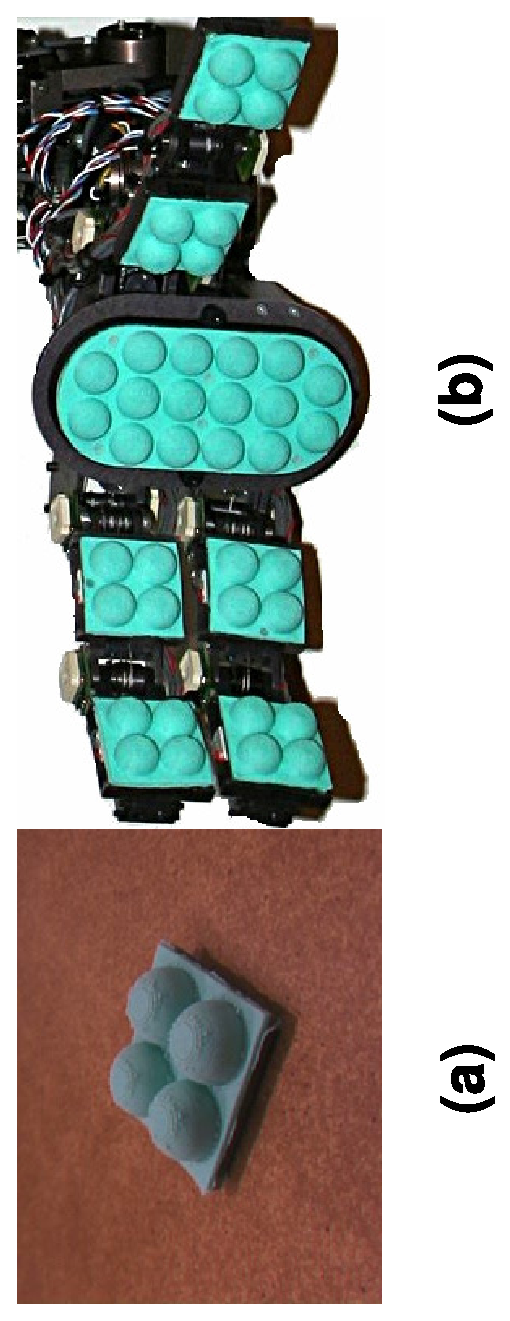
\includegraphics[width=1.0in, angle=270 ]{./figures/Tactiles.eps}
} \caption{Obrero's hand and detail of the tactile sensors. (a) Group of four tactile sensors. The
deformation of each of them is measured by a total of four sensors.
(b) Tactile sensors mounted on the hand.} \label{fig:TactileSensors}
\end{figure}

The tactile sensors mounted on the hand were designed to satisfy the
needs of robotic tasks. Each unit has a dome-like sensor (see
figure~\ref{fig:TactileSensors}a) made of silicon rubber. At the
tip of the dome we embedded a small magnet, whose position is
measured by four hall-effect sensors placed at the dome's base. By
sensing the position of the magnet the defomation of the dome
is estimated. The sensors are very sensitive and capable of 
detecting a minimum normal force of 0.098N. The shape of the sensors 
favors contact with the environment from any direction, as 
opposed to most of the tactile sensors which are
flat. The high deformability and the properties of the silicon
rubber allow the sensors to conform to the objects, thus
increasing friction and improving contact detection. 
%In this
%particular implementation, we used the ``magnetic'' version of
%these tactile sensors, however, an optical version has also been
%tested. 
The description of the design and the analysis of these
sensors can be found in \cite{etorresjSoft}.Groups of tactile 
sensors were placed on the hand. Two groups of four were placed 
on each finger (a group in each of the two
phalanges) and 16 on the palm. A detail of the palm and fingers
can be observed in figure~\ref{fig:TactileSensors}b. Each one of
these tactile units uses four sensors to determine the contact
forces. This means that overall the tactile feedback consists of
160 signals. At the base of the palm, where for practical reasons,
we were not able to mount these tactile sensors, we placed a
smaller infrared proximity sensor. To summarize, the hand has 5
motors, 8 DOF, 8 force sensors, 10 position sensors, 160 tactile
sensors and an infrared proximity sensor.

